\documentclass[a4paper, 11pt]{article} % Font size (can be 10pt, 11pt or 12pt) and paper size (remove a4paper for US letter paper)

%\usepackage[protrusion=true,expansion=true]{microtype} % Better typography
\usepackage{graphicx} % Required for including pictures
\usepackage{subfig}
\usepackage{wrapfig} % Allows in-line images

\usepackage{geometry}
\geometry{left=2.0cm,right=2.0cm,top=2.5cm,bottom=2.5cm}

\usepackage{mathpazo} % Use the Palatino font
\usepackage[T1]{fontenc} % Required for accented characters
\linespread{1.1} % Change line spacing here, Palatino benefits from a slight increase by default

\usepackage{hyperref}
\usepackage{amsmath}
\usepackage{color}
\newcommand{\reminder}[1]{\textbf{\color{red}[** #1 **]}}
\newcommand{\argmax}{\operatornamewithlimits{argmax}}
\newcommand{\argmin}{\operatornamewithlimits{argmin}}

\makeatletter

\renewcommand\@biblabel[1]{\textbf{#1.}} % Change the square brackets for each bibliography item from '[1]' to '1.'
\renewcommand{\@listI}{\itemsep=0pt} % Reduce the space between items in the itemize and enumerate environments and the bibliography

\renewcommand{\maketitle}{ % Customize the title - do not edit title and author name here, see the TITLE block below

\begin{flushright} % Right align
{\LARGE\@title} % Increase the font size of the title

\vspace{30pt} % Some vertical space between the title and author name

{\large\@author} % Author name
\\\@date % Date

\vspace{20pt} % Some vertical space between the author block and abstract
\end{flushright}
}

%----------------------------------------------------------------------------------------
%	TITLE
%----------------------------------------------------------------------------------------

\title{\textbf{Oversea Internship Final Report} % Title
} % Subtitle

\author{\textsc{Sida Gao} % Author
\\{Supervised by Prof. Emma Brunskill}
\\{\textit{Reinforcement Learning and Education Lab, CMU CSD}}} % Institutionz

\date{\today} % Date

%----------------------------------------------------------------------------------------

\begin{document}

\maketitle % Print the title section

%----------------------------------------------------------------------------------------
%	ABSTRACT AND KEYWORDS
%----------------------------------------------------------------------------------------

%\renewcommand{\abstractname}{Summary} % Uncomment to change the name of the abstract to something else

\begin{abstract}
This is the final report of my summer internship in CMU. It is \textit{NOT} a formal academic paper, since all of the projects pictured in this report are still works in progress. Therefore, some parts of the write-up won't be very formal, especially the reference part, which would only appear as footnotes (and works that are not that relevant would not be listed at all). This report assumes the readers have a general understanding of traditional AI, machine learning, deep learning and decision making, but will provide some backgrounds in reinforcement learning (RL), and educational data mining (EDM).

The main project for this summer is Deep Batch RL, in which I work with a master student, aiming to compare the generalization ability of model-based and model-free RL methods which both adopt deep learning models. Our original hypothesis believes that model-free methods should outperform the model-based ones, however, our emperical results suggest the opposite. The side project, in which I take the lead, focuses on extracting prerequisite relationships in educational data. This project also adopts deep learning models, which hold an advantage of dicovering complicated latent relations in the data over traditional methods. The last project I take part in is Adaptive Fraction, which aims to find robust tutoring policy with offline educational data collected from Fraction, an online tutor system. A robust policy is one we can expect it to be at least as good as our evaluations with simulated students. This project is currently at a rather preliminary phase and we are still working on designing and implementing the experiments.
\end{abstract}


\vspace{30pt} % Some vertical space between the abstract and first section

%----------------------------------------------------------------------------------------
%	ESSAY BODY
%----------------------------------------------------------------------------------------

\section{Introduction}

Artificial intelligents could be roughly divided into two classes: those that are trying to understand the world (classification, clustering, etc.) and those that are trying to improve the world with actions (decision making, planning, etc.). Reinforcement learning aims to do both, since it's trying to make optimal decisions in an unknown world. By doing some episodes of trials in the world, an RL agent collects trajectories of states (i.e. observations), rewards and actions. With these trajectories, the RL agent can pick the best action in any observed state, which would gain him the most reward. RL differs from decision making methods like Marcov decision processes, because MDPs have a perfect understanding and observation of the world, while RL agents know nothing about the transition model of states or the reward model (i.e., the rewards related to each state). In real life situations, the actual states are often not observable, and the agents would also need to learn to infer the states with observations.

Education, or to be more specific, intelligent tutor, is a perfect case where RL methods can be applied. We can easily draw some parallels between tutor systems and RL agents. The actions are the various tutoring materials that could be presented to students, while the rewards could be students' performance in tests. The world is also unknown: the transition model of students' knowledge states (i.e. how students would digest the materials) is unknown, and the reward model is also unknown (i.e. how student with a certain knowledge state would perform in a test). In education, we are also dealing with a partially observable environments, since we won't be able to directly see the knowledge state for students, and we can only have a belief state infered from observations of the students.

Education also poses an even larger challenge than other RL tasks. In conventional RL tasks like robotics, the robot can run trials in the real environments as much as we want, since in most cases the worst we can expect is merely a broken mechanical arm resulted from tripping over a stone. In education, it won't be ethical to collect online data on real students with an agent that's still learning from trials and errors. A crappy work-in-progress would do irreversible harms to real kids in this practice, and the things that could be broken would be the kids' future. Therefore, doing offline policy evaluation with trajectories collected from real world tutor systems (in which runs policies either designed by expert humans or well-tested AI agents) is an important track of research in educational RL.

Prof. Emma Brunskill's group, in which I interned for the summer, lies its interest in RL and education. We have shown that these two areas are intrinstically related. Our group covers a wide spectrum of research areas, from RL theories (machine learning) and traditional AI, all the way to more application oriented tracks like data mining and human computer interaction (in education). Given the special, yet not unique challenge of education described previously, our research projects are mostly focused on offline policy evaluation or planning. Educational data mining, which focuses on data collected from intelligent tutoring systems, is one of the may side interests of our group. Several distinctive characteristics of EDM include dealing with sequential data, and a special focus on discovering the latent hierarchical structure of data items (i.e. prerequisite structure of knowledge components). Deep learning, while has been widely adopted in various areas like computer vision, is still an emerging methods in RL and EDM, where only only a handful of previous works could be found. It is also a new area for the group.

In this section, we have briefly described the backgrounds and motivations of the projects. The following sections are organised as: section \ref{sec:DKT} described a deep learning model which my work in all 3 projects are based on; section \ref{sec:deepRL}, section \ref{sec:fraction} and section \ref{sec:influence} discusses the big pictures of the three projects, where we are and what part I play in them. At last, section \ref{sec:life} jots down some other aspects of the internship basides work, and section \ref{sec:summary} summarizes the 10-week internship.










\section{Deep Knowledge Tracing}
\label{sec:DKT}

\subsection{Knowledge Tracing Going Deep}

Knowledge tracing is a common task for educational data mining, with a goal towards accurately model the students' knowledge acquisition process. The conventional method, Bayesian Knowledge Tracing (BKT), keeps a binary state for each skill (i.e. knowledge component, or concept), either known or unknown. When a skill is not learned, by doing exercises on the skill, the student may have some probability to transition to the learned state. When answering a question on a certain skill, the student could get it wrong even when he already knows the skill (i.e. there exists a slip rate). And reversely, a student can get a question correct with luck, without knowing the skill, which corresponds to a guess rate. There have been various extentions to BKT, like modeling the forgetting process, and collapsing similar skills into one (since BKT tracks each skill separately, this kind of practice is trying to address the relations between skills).

There has been a quite influential work published in 2015, \textit{Deep Knowledge Tracing} \footnote{\textit{Deep Knowledge Tracing}, Chris Piech et al, NIPS 2015.} (DKT), which adopts an LSTM to model students' knowledge acquisition. Retrospectively speaking, LSTM is basically an upgraded version of BKT. Instead of having one binary state representation for each skill, LSTM uses a long vector of real numbers (which is normally more than the number of skills) to represent the knowledge state. By doing this, LSTM could capture complicated (and unfortunately, not very interpretable) relationships between different skills. The four gate layers in LSTM also closely resemble the key parameters in a BKT. The output gate, which reads out the hidden state vector to get an output (i.e. belief state on each skill), is a counterpart of slip and guess rate. The update gate, which scales the update value from the input, is like the acquisition rate. And the forget gate is literally modeling the forgetting of a knowledge component. In a nutshell, LSTM just upgrades the model of these processes from a single real number, to a layer of fully connected neural network. Therefore, we wouldn't be surprised to see DKT vastly outperforms BKT.

DKT can be simplified as a function approximator which takes a student's practice history (sequence of exercises he did, and whether he got each exercise correct or not) as input, and outputs the predictions (belief states) of the probability of getting each skill correct if presented as the next question.

\subsection{Implementing DKT}

DKT is a good modeling method for the student, i.e., a learned transition model of hidden knowledge states. This could be useful in various parts in our group's projects. Therefore, the first thing to do is implementing the model. 

Although there has already been several published DKT implementations, besides being a great opportunity to sort out all the subtlety like sequence padding and dropouts in LSTM, there are several other advantages of having our own implementation. First of all, our implementation is in Python, under the Tensorflow framework. Python is a friendly language for machine learning and data mining practices with its various powerful packages, and Tensorflow is a more flexible deep learning frame work, both of which provide convenience not presented in previous implementations. More importantly, our ultimate goal of DKT doesn't stop at getting a prediction metric on the test dataset, but to adopt it to do planning and data mining, thus calling an off-the-shelf LSTM cell from the framework won't work for us, since we won't be having access to the inner state of the LSTM that way. We need to implement the LSTM from scratch to better accustom to our goals. At last, since we have the full access to the model's structure, we made a small step forward of DKT by connecting the readout layer to the trainable initial state vector, which enables our DKT to predict the first answer without any previous input (which is a feature not presented in the original DKT implementation).

\subsection{Sanity Checks for DKT}

The biggest challenge of implementing a deep learning model is verifying the model. It requires little tuning (which is a great characteristic of using Adam optimizer in stochastic gradient descent) to get an AUC prediction performance comparable with previous works on the test set, however, we need more than a single AUC number to convince us that the model can be trusted.

Besides conventional checks like printing out or plotting several crucial variables/metrics, we did a more convincing sanity check. The goal is to test if DKT can fully recover a BKT model. First, we did a BKT simulation with 5 skills, each has its unique set of BKT parameters. As an extention to vanilla BKT, we add several prerequisite relations into the simulation: skill 0 and 1 are prerequisites for skill 2, while skill 2 and 3 are prerequisites for skill 4. We simulate such relations in a rather simplified manner: the student's acquisition rate of a skill would stay 0 until he learns all the prerequisites.

BKT model is actually a two-state HMM model, with acquisition rate corresponds to transition model, slip and guess rate corresponds to sensor model. Therefore, we can easily construct an oracle BKT inference model, which knows all the hidden parameters of BKT, and can infer the student's hidden knowledge state with the simulated trajectories as observations. A small tweak is needed to accustom to the prerequisite relations: the acquisition rate is an expected probability, conditioned on the knowledge states of prerequisites.

DKT can achieve the same AUC, 0.81, with this oracle BKT inference model. Again, only a AUC number won't be enough (there are millions of ways to accidentally get a high AUC). We computed the MSE (mean squared error) of the step-by-step belief states predicted by both models on the test set and got 0.003, which is a small number, but we still don't know if it's small enough. Therefore, we plot the knowledge tracing process given by the two models and compare the trends. From \ref{fig:match} we can see that DKT gives nearly identical predictions with oracle BKT. Combined with all the previous checks, we can safely say that our DKT model can be trusted and adopted in the projects.

\begin{figure}
\subfloat[DKT result on student 9999.]{
  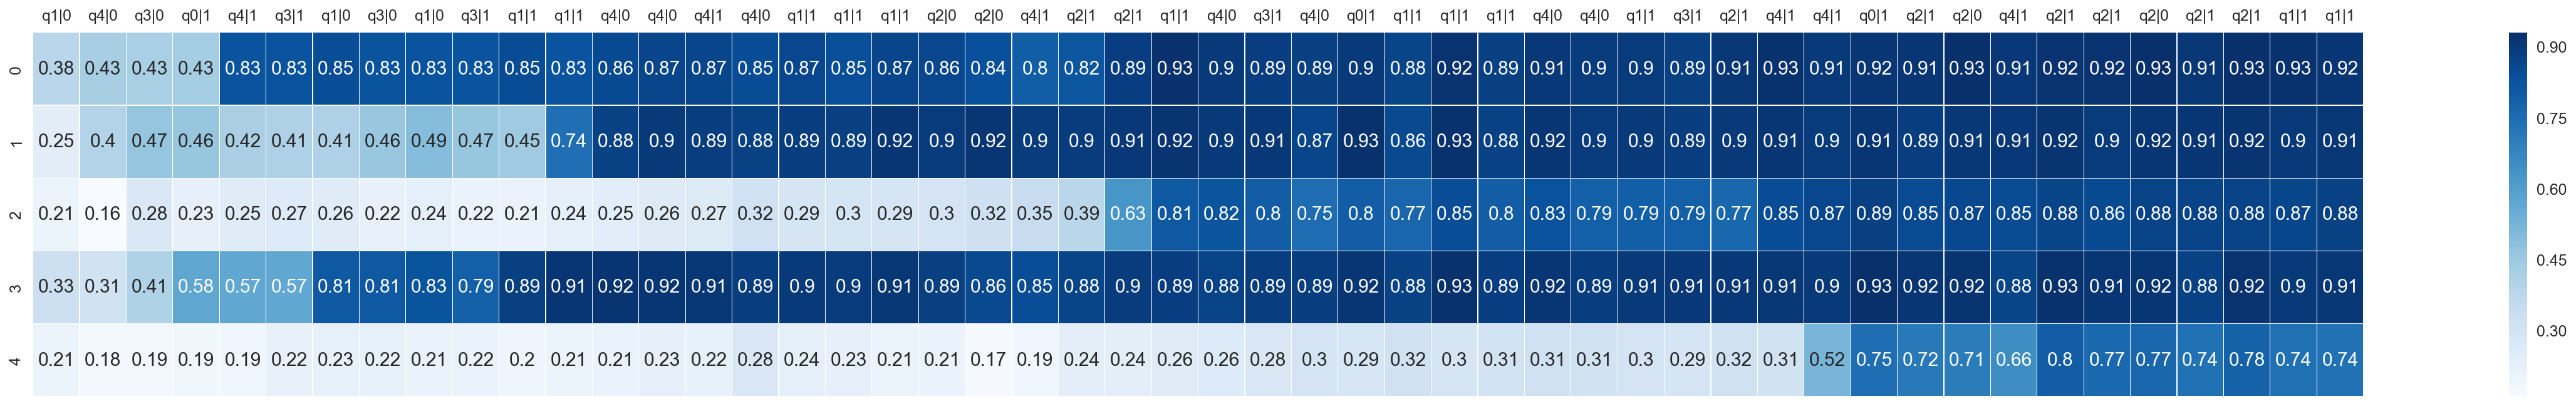
\includegraphics[width=1.0\linewidth]{figures/5th_dkt_9999.png}%
}
\newline
\subfloat[Oracle BKT result on student 9999.]{
  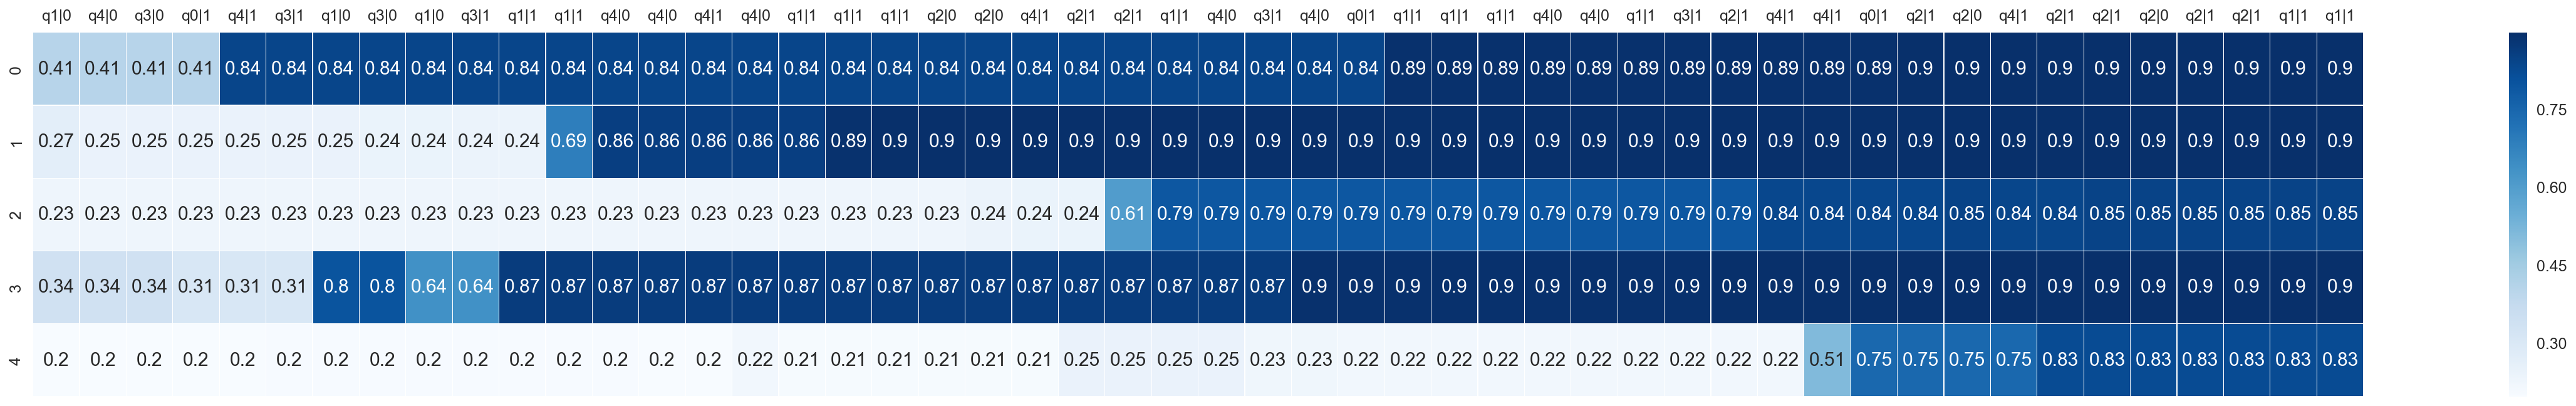
\includegraphics[width=1.0\linewidth]{figures/5th_bkt_9999.png}%
}
\caption{An example of the knowledge tracing visualization of DKT and BKT on one of the simualated student trajectory. The row labels are student ids. The column labels, $qi|j$, are student actions in each time step (with the leftmost action as the earliest): the question is on skill $i$, $j=1$ when the student answers correctly, otherwise $j=0$. Each column is the prediction for the action in the column label.}
\label{fig:match}
\end{figure}

In addition, we did a more novel sanity check, in which we reorder the train or test set in various ways and observe the consequenct AUC performance. This yields some interesting results and end up being a new project, which is ellaborated in section \ref{sec:influence}.

















\section{Deep Batch RL (for Education)}
\label{deepRL}

In this project, we want to compare two methods, the model-free method (DRQN) and the model-based method (expectimax search with DKT), both based on deep learning models, on off-policy learning for offline (i.e. a batch of) educational data. I focused on the model-based method, including its implementation and evaluation. The model-free method is done by Li Zhou, a graduate student in our group, and I was involved in the discussions of it.

\subsection{Model-based and Model-free RL}
\label{subsec:model-free}

In RL, our goal is to find the optimal policy in an unknown environment. There are mainly three ways of doing RL (the latter two are model-free methods, while we only focus on the comparison of the first two):

\begin{itemize}
\item First explicitly learn the model for the environment, i.e., the reward and transition model, then find the optimal policy using MDP (Markov Decision Process) method based on those.
\item Learn the Q values, i.e. the expected long-term utility of doing action $a$ in state $s$, $Q(s, a)$, without learning the environment model. With Q values, we can easily derive the optimal policy: $\pi(s)=\argmax\limits_a Q(s, a)$.
\item Directly learn the policy, i.e., we are directly mapping a state $s$ to an action $a$, without explicitly computing any model or utility. 
\end{itemize}

Our hypothesis is, model-free method should hold an advantage over model-based method in various aspects. First, a more apparrent one, model-free method is more computational feasible to scale-up, while doing MDP with a world model might involve tree searches, which is exponential. The more relevant advantage of a model-free method is that it's more sample efficient: you need a lot of samples to train an accurate world model (a slightly inaccurate model might suffer from an error explosion in the decision making process, thus result in a bad policy), but way less sample to simply know which action is better given the current state (i.e., no need to know the exact long-term utility).

\subsection{RL Going Deep}

\subsubsection{Deep World Model}

DKT is a good world model in education. It's a simple step forward to adopt DKT to do planning. With a DKT, we know the knowledge belief state for the student given any practice history, so we can evaluate any policy based on this.

To be more specific, we do a expectimax search with DKT. An expectimax seach tree has interleaving layers of max and expect nodes. A max node pick the children with the maximum value, while an expect node's value is an expectation of the value of its children. In our case, a max node will have children expect nodes each corresponding to an action (i.e. which skill to teach). An expect node will have children max nodes each corresponding to a possible probabilty for each outcome of the action (i.e., correct or incorrect). DKT can assign a probabilty to each outcome based on the observed history, thus an expectation can be computed over the children max nodes.

Unlike other tree search like minmax, expectimax tree could not be trimmed without a loss on the accuracy (since it's computing an expectation, and all the branch values are needed). Therefore, expectimax is expensive to compute (as is the case for most model-based algorithms).

Besides conventional speed-up coding tricks like minimize the function calls and the use of abstract classes, we specifically made an optimization for DKT. Since DKT does sveral matrix multiplications for each input vector, we can stack several vectors into an input matrix and compute the output simultaneously. This trick significanly reduces the computation time to the one sixth of the unstacked version.

\subsubsection{Deep Q-Learning}

Q-Learning, a model-free RL algorithm, is off-policy, which means that the policy we pick in updating and learning Q-values isn't necessarily the actual policy we run. The Q-values should satisfy equation \ref{eq:Q}, the Bellman function.

\begin{equation}
\label{eq:Q}
    Q(s,a)= R+\gamma\max\limits_{a'}Q(s',a'))
\end{equation}

where $R$ is the reward of state $s$, $\gamma$ is a discount factor for future's rewards, and other notations consistent with the description in \ref{subsec:model-free}. From this equation we can get a better understanding of off-policy: the $a'$ we pick is not the action that actually run, but the action than can maximize the Q value in state $s'$.

For discrete states we can simply put the Q values in a table and do value iterations until the Bellman functions are satisfied (close to iterative methods to solve linear equations). Yet we can't do that for continuous states as in our case, so we want to learn a parameterized function to approximate the Q function. Previous works have shown that this function approximation is not guaranteed to converge when it's not linear, especially when it's a neural network.

The Deep Q-Network\footnote{\textit{Human-level control through deep reinforcement learning}, Google DeepMind, 2016.} (DQN) adopts several ticks to resolve this diverging issue. DQN is an online (but still off-policy) algorithm, which does online exploration using $\epsilon-greedy$ search during training. Q-learning requires each update to be independant, thus when training the network, DQN employs an experience replay mechanism which feed randomized $(s, a, r, s')$ experience minibatches sampled from the pool of exploration history to the neural network. The loss that the neural network is minimizing is the difference of the left-hand and the right-hand size of equation \ref{eq:Q}.

The second trick is having a target network, which is identical to DQN but updated with a lower frequency. Since we are doing $\epsilon-greedy$ exploration, the distribution of data acquired during training is actually shifting, thus making the training very unstable (both sides of the Bellman equation is changing). If the two sides of the Bellman equation is provided by the same DQN, it would be like a dog chasing its own tail. The target network, however, can serve as a stable right-hand side of equation \ref{eq:Q}, thus resolve the diverging issue.

\subsubsection{Deep Recurrent Q-Learning}

The DQN deals with Atari games, where the state is fully observable from the consecutive 4 frames of the game. However, in our case, we are dealing with a partially observable environment, since we can only observe whether a student gets a problem correct, rather than their actual knowledge status. Therefore, we need to adopt an LSTM to map an action history (observations) to the Q-value. Previous work \footnote{\textit{Deep Recurrent Q-Learning for Partially Observable MDPs}, Matthew Hausknecht and Peter Stone, 2015.} has already added this extention to DQN, resulting in Deep Recurrent Q-Network (DRQN). However, in their work, the training of DRQN is still an online process.

Although DKT and DRQN both adopt an LSTM, both take the trajectory of students' actions as inputs, and even have the same number of outputs (one for each skill), they are very different function approximators (i.e. completely different loss functions). DKT's output is an approximate of the student's knowledge status, i.e. the probability of getting each skill correct, thus a supervised learning model (the result of the next question serves as the label). The output of DRQN is the long-term utility (i.e. rewards) of picking each skill as next action (i.e. question to give). Unlike DKT, the DRQN can be directly used to pick a policy. 

For real world data, besides being a comparison model of DRQN, another DKT instance, which is trained on a hold-out dataset unseen by DRQN or the expectimax-DKT, should serve as the "ground truth" for the evaluation of the policy picked by both DRQN and expectimax-DKT. However, we start with a comparison on BKT simualtion data, where the ground truth BKT model is known, thus a fair comparison between DRQN and expectimax-DKT.

\subsection{Challenges in Batch RL}

\subsubsection{Reward Function Design}

In any RL practice, we'll always face the challenge of how to properly define a reward function, since in most cases, the rewards would not be explicitly presented in ths data. A myopic or misspecified reward function might result in very undesirable outcomes\footnote{\textit{Concrete Problems in AI Safety}, Dario Amodei, Chris Olah, John Schulman, Jacob Stein- hardt, Paul Christiano, Dan Mane, 2016.}.

The reward function should be based on the trajectories in the data. We are not looking for myopic definitions like getting a reward whenever question is correctly answered (which would result in the agent constanly giving the same question to hack a high reward). Currently we are using a one-time-only reward associated to each skill, which is awarded once the student get 3 correct in a row.

In our DKT-expectimax framework, any trajectory based reward function can be swapped in. There are more variants of reward functions. A more natural one is to give a decaying reward for questions on the same skill. If we take the applicability into consideration, we probably should also give negative rewards for too many exercises on the same skill since we could run out of exercises in our pool. To make the training of DRQN more stable, we could also try giving awards only when trial ends, where some regularization may be needed. And we could also use discounted rewards, since we want to get rewards in the near future (the sooner the better).

\subsubsection{Constraints on Exploration}

In RL, when we talk about batch we mean offline (since we have a huge batch of fixed data to train on). For online RL, it’s single data entry (since we are constantly getting new data through greedy dearch) or mini-batch. We are doing an offline RL task, thus batch RL.

Several obstacles were encountered after we altered the DRQN into an offline version (the only difference is that we have a fixed pool for experience replay, while in the online version there are always new data coming into the pool). First, the model starts diverging before converging to the minimum loss. Second, though the model can achive its best performance (which is significantly higher than a random policy) when the loss is at its minimum, it cannot achieve a comparable performance with DKT-expectimax. Currently, the experiments of DKT are only restricted to the BKT simulated data (where we have the ground truth BKT). Table \ref{tb:planning} shows the comparison of different models and settings.

\begin{table}[]
\centering
\caption{Planning performances comparison. BKT and DKT models are used in a 5-step expectimax search for planning. The number of training instances is also listed. BKT-expectimax, with the BKT being the ground truth model, is the perfect policy. Random policy randomly picks a question at each time step, and serves as a baseline. (The 0.8 to 1.0 standard deviations are omitted in the table.)}
\label{tb:planning}
\begin{tabular}{|c|c|}
\hline
Algorithm       & Average rewards after a 20 problem episode \\ \hline
BKT             & 2.6                                        \\ \hline
DRQN \#ins=5000 & 2.1                                        \\ \hline
DKT \#ins=5000  & 2.6                                        \\ \hline
DKT \#ins=100   & 2.28                                       \\ \hline
Random          & 0.94                                       \\ \hline
\end{tabular}
\end{table}

As we have shown in section \ref{sec:DKT}, DKT can fully recover the BKT, so we are not surprised to see that a fully-trained DKT (with 5000 instances) can gain an optimal policy. However, in real world, we shouldn't expect DKT to fully recover the underlying model of real students. To better simulate this situation, we train DKT with little data (merely 100 instances). With this DKT, both the AUC on test set and the performance of its policy suffer a huge drop (which is consistent with our prior hypothesis, that DKT's performance is vulnerable to data available). 

However, even an inaccurate DKT like that still outperforms DRQN, and in this case DRQN is trained on way more data. This greatly conflicts our prior hpothesis, since DRQN should be more sample efficient and unless the myopic expectimax which can only look 5 steps ahead (when keeping the computation feasible), DRQN's Q-value estimation is infinite horizon (i.e. looks infinite steps ahead). 

We've tried several tricks and fine tuning for DRQN. For example, for offline training, the data distribution is fixed, so maybe we don’t need a target network like the online DQN. However, emperically, the trickes we have tried don’t make a difference.

The breakthrough finding came when we modify the algorithm to online (which is only possible for simulation since we need the ground truth simulator) it can perform on par with the optimal policy. When we do greedy search, it converges fast (because we have a lot of near-optimal sequences), while when we do completely random search, the performance drops after a short boost (just like the offline performance), then come back to the optimal performance eventually, which could be mainly due to the massive (around $10^5$ episodes) random dataset (in which there are enough good/near-optimal examples) that has already added in the pool. Greedy search is basically changing the training dataset, so we can easily accept the fact that it’s way better.

The current drawback of offline DRQN is clear: unable to do exploration, thus require a massive amount ($10^5$ episodes) of random data to see enough near-optimal trajectories. On the contrary, DKT can easily pick up a vague prerequisite structure even under a small dataset (100 episodes), by observing that some skills are easier to learn in the begining while others are not. Based on this little knowledge, the expectimax can get us an optimal policy. In this current setting, model-based method seems to win on planning performance (especially when model-free method is not that sample efficient as we thought it should be).

\subsection{Future Work}

Experimantal results so far have shown that deep batch Q-learning possibly couldn't work due to the inability of doing exploration in the environment. It turns out that the generalization ability of deep neural network is not that powerful as we expected. However, we are still trying to fine tune the DRQN to see if its performance could go up. A more promising direction is to integrate return based off-policy RL algorithms \footnote{\textit{Safe and Efficient Off-Policy Reinforcement Learning}, Remi Munos, Tom Stepleton, Anna Harutyunyan, Marc G. Bellemare, 2016.} into deep RL. This has not been done by any previous work before thus we might be on to something really innovative.

There are several concerns on the current experiment setting on simulation though. We only have 20 trials for each episode, i.e. our horizon is fairly short. A method as shallow as DKT-expectimax (5 steps look ahead) can perform as near-perfect because we can only expect the students to learn those skills without prerequisites. If we have a setting where a shallow sight might be catastrphic (like a longer horizon and a more complicated skill structure, with loose prerequisite relations as in the real world), we might see DRQN to win, since it can look infinite steps. However, none of these could account for the low performance of DRQN on the simpler simulation data (it should be able to get the optimal policy).

A minor technical issue we need to point out here. First, currently the model-based method is technically not a real RL algorithm, since the reward model is not learned but directly coded in the tree search algorithm. We can use something like DKT to learn the model, but in this case it would be a regression task rather than a classification one. The fix won't be easy and is not going to help with our main concern (why DRQN is underperforming) either.

There are more interesting directions that we have in mind, including planning with multi-skill questions and making sense of the necessary horizon length for getting an optimal policy (in extreme cases like all the skills are independent, pick any skill wouldn't make a difference, thus zero horizon is as good as infinite horizon). As for application, we should also account for a certain dropout rate when searching for policy. If a student drops out in the middle, a short horizon might be better, since the long-term benefits we planned for the student might not pay off. These thoughts are even more off-topic, and could be discussed in future projects.
\section{Adaptive Fraction}
\label{sec:fraction}

This project, Adaptive Fraction, is led by another graduate student in our group, Shayan Doroudi.
Our group has some collaboration with an HCI group at CMU, and we run an online intelligent tutor system, Fraction, which tutors grade school level math (on fraction). With this system, we can deploy experiments on real students. However, as we have mentioned before, we want to make sure that our policy would be robust, which means that when we deploy it on our system, we should be sure that the result won’t be worse than what we evaluated in (offline) experiments. 

\subsection{Robust Policy}

There are many methods to model a student's knowledge acquisition process, DKT being one of them. Our assumption is, some of these models (or at least some part of it) is correct, and the result can be partially trusted. However, if we only adopt one student model, we might end up with an overfitted policy on this model, and might have negative consequences on real students.
Therefore, we need to see what the best or worst our policy could do on various student models.

We will have a matrix to show how different policies (which could be built on one of the student models or worlds) can perform on different worlds. DKT could serve as one world, and expectimax is one way to learn a policy on this world. The matrix would have world and policy as its two axes, and performance as its values. We expect to see that the values on diagnal be higher (since diagnal values correspond to the performance of policies tested on the same world that generated the policy in the first place), and hope to find a policy that's good on all world models. Shayan has already implemented a framework of testing policies on different worlds. My job is to port my DKT implementation, and its simulation code into his framework. DKT has a fairly good AUC, 0.81, on the Fraction dataset.

\subsection{Future Work}

It's possible to incorporate expectimax with DKT as a policy as well. However, the Fraction dataset's structure is more complicated than simulation or other real datasets: instead of having a single latent skill, each problem consists of multiple steps; students will only meet the same problem once, but different problems can share same steps; different steps within the same problem can have different results; each step is associated with a skill. Therefore, by taking an action (picking a problem), there are $2^{num\_steps}$ possible outcomes, thus expect node would have more children. And the possibility associated with each max node (as a child of expect node) need to come after a multiple step simulation of DKT. We are not sure if we are going to need DKT-expectimax in the framework though, since it would be prohibitive to even look ahead 3 steps (thus very myopic).

In Fraction, after exercises (a tutor session), the student will do a post test. Post test score is our reward. Besides student models, we also use the data to train a reward model. We first feed the tutor session trajectory to a student model, then use the final belief state to do a LASSO regression (linear regression with L1 regularization) on post test score, which gives us the reward model. However, this method gives nearly identical predictions for all policy-world combinations. So one of the major next steps we are thinking is to combine the student and reward model as one (so that we can directly predict the posttest performance given the within-tutor trajectory). This probably would require some tweak to the DKT.

As an extention to the matrix, we are also planning to train student models on a subset of students (above or below average students). Moreover, my implementation of the loose-prerequisite BKT model (with different sets of parameters for different numbers of mastered prerequisites) could be integreted in the framework as well. The current BKT inference model didn't fully leverage the prerequisite structure, since it doesn't update the children or ancestor's belief when encounters a skill. There are still some math to work out for this upgrade.

\section{Influence of Skill Orders}


follow ups of DKT, traditional outperform

DKT no domain knowledge is required

Data quality issues


\section{Summary}
\label{sec:summary}

During the past ten weeks, my project started out as repeating a published model and ended up with some new exciting directions to explore. Besides my hands-on experiments, I also participated in a lot paper reading and discussion on RL in the group, which got me acquainted to a whole new area and a group of interesting people.

This ten-week internship has been deeply rewarding. As a college-senior-to-be, I've never been more capable of doing research and I've never gotten the opportunity of fully devoting myself to research for such a long time span. This experience has been exhausting and mad fun at the same time, and it further established my mind to be a researcher, and a truth seeker.

\end{document}